\scanpage{37}
\margin{?\quad\figure{\begin{tikzpicture}\draw (0,0)--(0,1.4);\end{tikzpicture}}}
Une question plus subtile est s'ils peuvent s'inverser, quand c'est des isomorphismes\ldots.

\uline{Dualité} entre \(P^i(X)\) et \(P^{\deleted{n+1-i}\inserted{j}}(X)\) \inserted{pr \(i+j=n+1\)} : Si \(A,B\) \deleted{\unsure{les}} \deleted{\unsure{unes}}\inserted{des} VA, \deleted{dont la dualité est} accouplées pr une dualité parfaite \((A\simeq\unsure{B'|B^*},B\simeq A^*)\), alors il y a correspondance biunivoque entre \(\operatorname{Hom\,alg}(A,P^i(X))\) et \(\operatorname{Hom\,alg}(P^{\unsure{j|1}}(X),B)\).

En effet, si on a un hom \(A\longrightarrow P^i(X)\), défini pr un \(Z\in A^i_{\mathrm{alb}}(X\times A)\), alors \({}^tZ\) définit un hom
\diagram{\begin{tikzcd}[ampersand replacement=\&]
P^j(X)\arrow[r]\&P^{i+j-n}(A)=P^1(A)\arrow[d,phantom,"\simeq" rotate=90]\\
\&B
\end{tikzcd}}
et inversement si on a \(P^j(X)\longrightarrow B\). \deleted{Notations}\inserted{Cependant,}
\deleted{\(\unsure{{}^t\varphi=\varphi^t}\). Plus généralement}
il faut vérifier que \(P^j(X)\longrightarrow B\) ne dépend que de l'\uline{application} \(A\longrightarrow P^i(X)\), pas du cycle \(Z\).
\margin{\figure{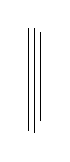
\begin{tikzpicture}[x=1cm,y=1cm]\draw (0,0)--(0,1.3);\draw (.08,-.03)--(.08,1.3);\draw (.16,.12)--(.16,1.25);\end{tikzpicture}}}

Question de transposition se pose, plus généralement, pr \(P^i(X)\mathbin{-}P^{i'}(X')\) en \(P^{j'}(X')\mathbin{-}P^j(X)\).

Cf plus bas\ldots.
\mspage{36}
